\documentclass{article}
\title{支持向量机}
\author{QwanxingxuA}
\usepackage{ctex}
\usepackage{amsmath}
\usepackage{amssymb}
\usepackage{graphicx}
\usepackage{float}
\begin{document}
\maketitle
\part{线性可分支持向量机与硬间隔最大化}
    \section{简述}
        线性可分支持向量机的思想在感知机那一章已经讨论了很多，笔者从策略的角度重点探讨了损失函数方法。本Part将
        从函数间隔、几何间隔的角度严格推导感知机那一节论述的思想。考虑本文仅是学习推导，不是严格的数学专著，相关前提定义
        在感知机文档中已经给出，本文不再重复定义，直接使用。
    \section{函数间隔与几何间隔}
        对于给定数据集$D$和超平面$(\boldsymbol{w},b)$，假设超平面$(\boldsymbol{w},b)$可以正确分类数据集$D$。

        超平面$(\boldsymbol{w},b)$关于样本$(\boldsymbol{x}_i,y_i)$的函数间隔：
        \[\widehat{\gamma }_i=y_i(\boldsymbol{w}\cdot \boldsymbol{x}_i+b)\]
        
        超平面$(\boldsymbol{w},b)$关于数据集$D$的函数间隔：
        \[\widehat{\gamma} =\min_{i=1,2,\dots,n}\widehat{\gamma}_i\]

        超平面$(\boldsymbol{w},b)$关于样本$(\boldsymbol{x}_i,y_i)$的几何间隔：
        \[\gamma_i =\frac{y_i(\boldsymbol{w} \cdot \boldsymbol{x}_i+b)}{\|\boldsymbol{w}\|}\]

        超平面$(\boldsymbol{w},b)$关于数据集$D$的几何间隔：
        \[\gamma=\min_{i=1,2,\dots,n}\gamma_i\]

        实际上，这里的两种间隔就对应于感知机中讨论的两种策略（感知机考虑的是分类错误的样本）。函数间隔会随参数等比例缩放而改变，不具备尺度不变性；几何间隔消除了参数缩放带来的影响，定义唯一。
        从置信度的角度考虑，几何间隔衡量了分类正确的置信程度。对应感知机章节的结论：几何间隔不只要求样本越过分界超平面，还要将样本到超平面的距离纳入评价，这点后续优化问题会进一步体现。

        更深入的说，两种优化目标对应不同策略，对泛化误差带来不同影响。之前论述过，不同的策略会影响泛化误差及其上界。
        函数间隔仅保证样本分类正确；几何间隔追求更大的分离余量，模型泛化能力更强。换言之，几何间隔最小化策略对应的风险误差或者其上界在概率意义上更小。

        最后要强调一点，不能直接把感知机思路完全套用到支持向量机。虽然函数间隔、几何间隔的概念一致，但感知机是以误分类样本为出发点；
        线性可分SVM建立在所有样本分类正确的前提之上开展优化。

    \section{间隔最大化}
        基于上述讨论，可以给出基于几何间隔最大化的优化问题：
        \begin{align*}
            \max \quad & \gamma \\
            s.t. \quad & \frac{y_i(\boldsymbol{w}\cdot \boldsymbol{x}_i+b)}{\|\boldsymbol{w}\|}\ge \gamma,\quad i=1,2,\dots,n
        \end{align*}

        代入几何间隔定义，问题可以转换为：
        \begin{align*}
            \max \quad & \frac{\widehat{\gamma}}{\|\boldsymbol{w}\|}  \\
            s.t. \quad & y_i(\boldsymbol{w}\cdot \boldsymbol{x}_i+b)\ge \widehat{\gamma},\quad i=1,2,\dots,n
        \end{align*}

        由于超平面具备尺度不变性：若$(\boldsymbol{w},b)$是可行解，则对任意$k>0$，$(k\boldsymbol{w},kb)$对应同一超平面，函数间隔同步缩放$k$倍。因此$\widehat{\gamma}$的取值不影响该问题最优解，我们可以人为归一化取$\widehat{\gamma}=1$：
        \begin{align*}
            \max \quad & \frac{1}{\|\boldsymbol{w}\|}  \\
            s.t. \quad & y_i(\boldsymbol{w}\cdot \boldsymbol{x}_i+b)\ge 1,\quad i=1,2,\dots,n
        \end{align*}

        最大化$\dfrac{1}{\|\boldsymbol{w}\|}$等价于最小化$\dfrac{1}{2}\|\boldsymbol{w}\|^2$，问题转换为：
        \begin{align*}
            \min \quad & \frac{1}{2}\|\boldsymbol{w}\|^2  \\
            s.t. \quad & y_i(\boldsymbol{w}\cdot \boldsymbol{x}_i+b)\ge 1,\quad i=1,2,\dots,n
        \end{align*}

        到此便将原问题转换为典型的凸二次规划问题。书中直接假设最优解下一定存在样本使得约束取等，初次阅读容易产生疑惑：为什么最优解必然落在约束边界？
        关键结论：目标函数$\dfrac12\|\boldsymbol{w}\|^2$是严格凸函数，可行域为凸集；严格凸优化问题的最优解必然位于可行域边界。
        直观理解：若某组可行解全部约束严格大于1，我们可以等比例缩小$\|\boldsymbol{w}\|$，进一步优化目标，因此内部点不可能成为最优解。

        下面证明几何间隔最大化问题最优解$(\boldsymbol{w}^*,b^*)$存在且唯一。

        (1)存在性
        上述问题可行域由一组线性不等式约束构成，是凸集；目标函数为二次正定函数，强制有下界。因此该凸优化问题一定存在最优解
        $(\boldsymbol{w}^*,b^*)$。

        (2)唯一性
        假设存在两个不同最优解$(\boldsymbol{w}_1,b_1),(\boldsymbol{w}_2,b_2)$，满足$\|\boldsymbol{w}_1\|=\|\boldsymbol{w}_2\|=c$。令$\boldsymbol{w}=\dfrac{\boldsymbol{w}_1+\boldsymbol{w}_2}{2}$，由三角不等式：
        \[c\le \|\boldsymbol{w}\| \le \frac{\|\boldsymbol{w}_1\|+\|\boldsymbol{w}_2\|}{2} =c\]
        
        上式取等号成立的充要条件是$\boldsymbol{w}_1,\boldsymbol{w}_2$同向共线，因此：
        \[\boldsymbol{w}^*=\boldsymbol{w}_1=\boldsymbol{w}_2\]

        设最优超平面正负间隔边界上分别存在支持向量$\boldsymbol{x}'$（正类）、$\boldsymbol{x}''$（负类），则：
        \[b_1=-\frac{1}{2}(\boldsymbol{w}^*\cdot \boldsymbol{x}'_1+\boldsymbol{w}^*\cdot \boldsymbol{x}''_1)\]
        \[b_2=-\frac{1}{2}(\boldsymbol{w}^*\cdot \boldsymbol{x}'_2+\boldsymbol{w}^*\cdot \boldsymbol{x}''_2)\]

        于是
        \[b_1-b_2=-\frac{1}{2}\boldsymbol{w}^*\cdot\big[(\boldsymbol{x}'_1-\boldsymbol{x}'_2)+(\boldsymbol{x}''_1-\boldsymbol{x}''_2)\big]\]

        又由约束条件：
        \[\boldsymbol{w}^*\cdot \boldsymbol{x}'_2+b_1 \ge 1 =\boldsymbol{w}^*\cdot \boldsymbol{x}'_1+b_1\]
        \[-(\boldsymbol{w}^*\cdot \boldsymbol{x}''_2+b_1) \ge 1 =-(\boldsymbol{w}^*\cdot \boldsymbol{x}''_1+b_1)\]

        推得
        \[\boldsymbol{x}'_1=\boldsymbol{x}'_2,\quad \boldsymbol{x}''_1=\boldsymbol{x}''_2\]
        \[b_1-b_2=0\]

        综上：
        \[(\boldsymbol{w}_1,b_1)=(\boldsymbol{w}_2,b_2)\]
        
        证毕！

        到此便可以引入支持向量概念。如下图，边界$\boldsymbol{w}\cdot \boldsymbol{x}+b=\pm 1$构成两条间隔边界$H_1$、$H_2$，它们之间
        的距离是$\dfrac{2}{\|\boldsymbol{w}\|}$。可以试想，若归一化不取1，仅带来参数整体缩放，超平面与间隔距离保持不变，
        本质等价，这也印证了前面尺度不变性的结论。
        \begin{figure}[h]
        \centering
        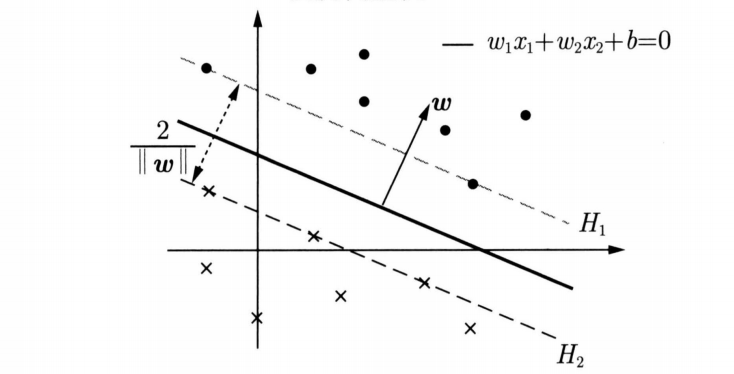
\includegraphics[width=0.6\textwidth]{支持向量.png}
        \caption{支持向量示意图}
        \label{fig:svm-sv}
        \end{figure}
    \section{对偶算法}
        对偶算法是最优化的一种方法，上述基于几何间隔策略得到原始最优化问题。这个问题具有很好的特性：约束函数满足
        凸性；该问题满足强对偶性。更好的消息是KKT条件支撑了超平面的确立。

        构建拉格朗如函数：
        \[L(\boldsymbol{w},b,\boldsymbol{\alpha })=\frac{1}{2}\|\boldsymbol{w}\|^2 +\sum_{i=1}^{n}\alpha_i[(1-y_i(\boldsymbol{w}\cdot \boldsymbol{x}_i+b))]=\frac{1}{2}\|\boldsymbol{w}\|^2-\sum_{i=1}^{n}\alpha_iy_i(\boldsymbol{w}\cdot \boldsymbol{x}_i+b)+\sum_{i=1}^{n}\alpha_i \]
        
        其中,$\boldsymbol{\alpha}=(\alpha_1,\alpha_2,\cdots,\alpha_n)^T$是拉格朗日乘子向量。

        对偶问题是极大极小化问题，先解极小化问题：
        \[\nabla_{\boldsymbol{w}}L=\boldsymbol{w}-\sum_{i=1}^{n}\alpha_iy_i\boldsymbol{x}_i=0\]
        \[\nabla_bL=\sum_{i=1}^{n}\alpha_iy_i=0\]
        \[\Rightarrow \boldsymbol{w}=\sum_{i=1}^{n}\alpha_iy_i\boldsymbol{x}_i,\quad\sum_{i=1}^{n}\alpha_iy_i=0\]
        
        代回拉格朗日函数得到极大化问题：
        \[\max_{\boldsymbol{\alpha}}\quad-\frac{1}{2}\sum_{i=1}^{n}\sum_{j=1}^{n}\alpha_iy_i\alpha_jy_j(\boldsymbol{x}_i\cdot \boldsymbol{x}_j)+\sum_{i=1}^{n}\alpha_i\]

        将上述问题转换为标准形式：
        \begin{align*}
            \min_{\boldsymbol{\alpha}}\quad & \frac{1}{2}\sum_{i=1}^{n}\sum_{j=1}^{n}\alpha_iy_i\alpha_jy_j(\boldsymbol{x}_i\cdot \boldsymbol{x}_j)-\sum_{i=1}^{n}\alpha_i\\
            s.t. \quad & \sum_{i=1}^{n}\alpha_iy_i=0 \\
                       & \alpha_i \ge 0,\quad i=1,2,\cdots,n
        \end{align*}

        解决这个最优化问题得到最优解$\boldsymbol{\alpha}^*,\boldsymbol{w}^*,b^*$。依据最优化理论，它们分别是对偶问题和
        原始问题的最优解。通过KKT条件可以得到原始问题的具体解：

        KKT部分条件：
        \[\boldsymbol{w}-\sum_{i=1}^{n}\alpha_iy_i\boldsymbol{x}_i=0\]
        \[\alpha_i^*[1-y_i(\boldsymbol{w}\cdot\boldsymbol{x}_i+b)]=0,\quad i=1,2,\cdots,n\]
        \[\boldsymbol{\alpha}_i^* \ge 0,\quad i=1,2,\cdots,n\]

        一定存在$\boldsymbol{\alpha}_j^*=0$。通过反证法证明，假设不存在，那么$\alpha^*=0$，于是$\boldsymbol{w}^*=0$。代入原始问题
        发现这不是最优解，假设不成立。

        结合第二个KKt条件可以得到：
        \[1-y_j(\boldsymbol{w}\cdot \boldsymbol{x}_j+b)=0\]

        考虑到$y_i^2=1$的特性：
        \[b=y_j-\boldsymbol{w}\cdot\boldsymbol{x_j}\]

        整理出来得到超平面
        \[(\sum_{i=1}^{n}\alpha_iy_i\boldsymbol{x}_i \quad,\quad y_j-\sum_{i=1}^{n}\alpha_iy_i(\boldsymbol{x}_i\cdot\boldsymbol{x_j}))\]

        基于KKT条件我们发现会出现样本满足$y_i(\boldsymbol{w}^*\cdot \boldsymbol{x}_i+b^*)=1$,它们便是支持向量。

\part{线性支持向量机与软间隔最大化}
    \setcounter{section}{0}
    \section{线性支持向量机}
        线性支持向量机针对线性不可分数据。通常情况下可以将噪声或者特异点去除通过线性可分支持向量机解决。线性支持向量机
        可以直接处理，这点与感知机有点类似，但一定要注意感知机是无法突破线性的，多层感知机是可以突破线性的。

        线性支持向量机添加松弛变量$\xi$。松弛变量这个名称取得非常形象，在当下问题就是将线性分开的限制松弛一点，从数学
        的角度上看是将线性可分支持向量机中的约束松弛一点，即$y_i(\boldsymbol{w}\cdot\boldsymbol{x}_i)\ge 1-\xi_i$。但松弛肯定不能过度，于是
        加上惩罚性来限制松弛，这点与正则化是一致的。于是可以得到最优化问题：
        
        \begin{align*}
            \min_{\boldsymbol{w},b,\boldsymbol{\xi}} \quad & \frac{1}{2}\|\boldsymbol{w}\|^2+C\sum_{i=1}^{n}\xi_i,\quad i=1,2,\cdots,n\\
            s.t. \quad & y_i(\boldsymbol{w}\cdot\boldsymbol{x}_i)\ge 1-\xi_i,\quad i=1,2,\cdots,nabla\\
                    &   \xi_i \ge 0,\quad i=1,2,\cdots,n
        \end{align*}
        后续同线性可分支持向量机一致，不在赘述。

    \section{对偶算法}
    构造拉格朗如函数：
    \[L(\boldsymbol{w},b,\boldsymbol{\xi},\boldsymbol{\alpha},\boldsymbol{\mu })=\frac{1}{2}\|\boldsymbol{w}\|^2+C\sum_{i=1}^{n}\xi_i-\sum_{i=1}^{n}\alpha_iy_i(\boldsymbol{w}\cdot\boldsymbol{x}_i+b)+\sum_{i=1}^{n}\alpha_i(1-\xi_i)-\sum_{i=1}^{n}\mu_i\xi_i\]

    通过解决极小化问题得到：

    \begin{align*}
        \min_{\boldsymbol{\alpha},\boldsymbol{\mu}} \quad & \frac{1}{2}\sum_{i=1}^{n}\sum_{j=1}^{n}\alpha_iy_i\alpha_jy_j(\boldsymbol{x}_i\cdot\boldsymbol{x}_j)-\sum_{i=1}^{n}\alpha_i \\
        s.t.    \quad & \sum_{i=1}^{n}\alpha_iy_i=0\\
        &   0\le \alpha_i \le C,\quad i=1,2,\cdots,n 
    \end{align*}

    这里的最后一个约束实际上是原本多个约束的等价形式。

    通过KKt条件可以得到：
    \[\boldsymbol{w}^*=\sum_{i=1}^{n}\alpha_iy_i\boldsymbol{x}_i\]
    \[\alpha_i^*[1-\xi_i-y_i(\boldsymbol{w^*}\cdot\boldsymbol{x}_i+b^*)]=0,\quad i=1,2,\cdots,n\]
    \[\mu_i^*\xi_i=0,\quad i=1,2,\cdots,n\]
    \[C-\alpha_i-\mu_i=0,\quad i=1,2,\cdots,n\]

    如果存在$0<\alpha_j< C$,则$b^*=y_j-\sum_{i=1}^{n}\alpha_iy_i(\boldsymbol{x_i}\cdot\boldsymbol{x}_j)$，注意这里要结合最后一个KKT条件。
    
    如果$\alpha_j=C$，若$0<\xi_i<1$,则分类正确；若$\xi_i=1$，则在超平面上；若$0<\xi_i>1$，则分类错误，
    这实际是该问题的支持向量，可见下图。
    
    \begin{figure}[H]
        \centering
        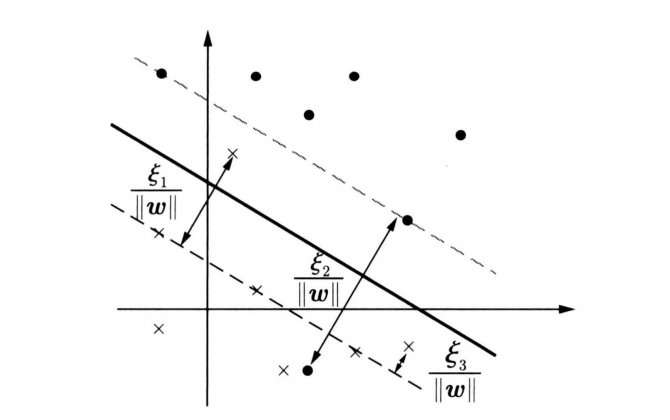
\includegraphics[width=0.8\textwidth]{线性支持向量.png}
        \caption{线性支持向量}
    \end{figure}

    \subsection*{等价形式与感知机对比分析}
        对偶问题具有等价的形式,即合页损失函数：

        \[\min_{\boldsymbol{w},b}\quad \sum_{i=1}^{n}[1-y_i(\boldsymbol{w}_i\cdot\boldsymbol{x_i}+b)]_++\lambda \|\boldsymbol{w}\|^2\]

        令$[1-y_i(\boldsymbol{w}_i\cdot\boldsymbol{x_i}+b)]_+=\xi_i$得到等价形式：
        \[\min_{\boldsymbol{w},b,\boldsymbol{\xi}}\quad \sum_{i=1}^{n}\xi_i+\lambda\|\boldsymbol{w}\|^2\]

        令$\lambda=\frac{1}{2C}:$

        \[\min_{\boldsymbol{w},b,\boldsymbol{\xi}}\quad \frac{1}{C}(C\sum_{i=1}^{n}\xi_i+\frac{1}{2}\|\boldsymbol{w}\|^2)\]

        从策略角度看，这是将分类错误纳入经验误差。模型希望减少错误分类，有感知机的意思。实际上
        感知机也可以写成上述形式：
        \[\min_{\boldsymbol{w},b} \quad [y_i(\boldsymbol{w}\cdot\boldsymbol{x}_i)]_+\]

        可以发现软间隔考虑了确信度，这与前文感知机与支持向量机对比分析相印证。
        
\part{核函数}
    \setcounter{section}{0}
    \section{核技巧}
        对于非线性分类问题，线性支持向量机难以解决，这时候可以利用核技巧。方法本身
        是将原始空间映射到新空间，使数据在新空间是线性可分的。
        定义映射
        \[\phi :\mathcal{X}  \rightarrow \mathcal{H} \]
        
        由线性支持向量机可知，决策函数：
        \[f(x)=sign(\sum_{i=1}^{n}\alpha_iy_i(\phi(x_i)\cdot\phi(x))+b)=sign(\sum_{i=1}^{n}\alpha_iy_iK(x_i,x)+b)\]

        关于核函数，离散数学有介绍。这里的关键是要满足$\mathcal{H}$是希尔伯特空间，因为如果没有内积上式不成立。

        核技巧的思想是不显式定义映射$\phi$，直接定义核函数。所以现在的问题是如何定义核函数以及如何判断定义的函数是不是核函数。
        从方法是看很简洁，通过构造法构造一个希尔伯特空间即可。具体步骤是通过线性组合构造一个向量空间，即满足数乘和加法封闭，然后
        构造内积运算，最后完备化得到希尔伯特空间。这里面涉及离散数学、泛函分析等，证明略，可以得到结论：

        设$K:\mathcal{X} \times  \mathcal{X} \rightarrow \mathsf{R} $是对称函数，则$K(x,z)$为正定核函数的充要条件是对任意
        $x_i \in \mathcal{X},\quad i=1,2,\cdots,m,K(x,z)$对应的Gram矩阵
        \[K=[K(x_i,x_j)]_{m \times m}\]
        是半正定的。

        基于上述结论，该问题变得很简洁了，只需要重点关注Gram矩阵即可。但是数据很大的时候，验证是很不容易的，所以常见的方法是直接利用已经
        完备的核函数，下面列举几种常见的核函数：

        多项式核函数：
        \[K(x,z)=(x\cdot z+1)^p\]

        高斯核函数：
        \[K(x,z)=\exp(-\frac{\|x-z\|^2}{2\sigma ^2})\]

    \section{SMO算法}
        假设已经找到前文所述的核函数$K$。基于线性支持向量机，得到如下优化问题：
        \begin{align*}
            \min_{\boldsymbol{\alpha}} \quad & \frac{1}{2}\sum_{i=1}^{n}\sum_{j=1}^{n}\alpha_i\alpha_jy_iy_jK_{ij}-\sum_{i=1}^{n}\alpha_i \\
            s.t. \quad & \sum_{i=1}^{n}\alpha_iy_i=0, \\
            & 0 \le \alpha_i \le C,\quad i=1,2,\cdots,n
        \end{align*}
        
        其中$K_{ij}=K(x_i,x_j)$。

        该优化问题可以通过KKT条件解决。如果全部满足KKT条件，那显然找到了最优解，相反则至少存在一个变量不满足KKT条件。
        SMO方法选取两个变量，其中至少一个变量不满足KKT条件。解决子问题，让目标函数降低，由最优化理论知道，变量也会向满足KKT条件
        靠近。实际上这种方法在最优化理论里面很多，诸如有效集。其核心思想是解决子问题，因为子问题相比于大问题好解决的多。

        假设选定$\alpha_1,\alpha_2$,有子问题
        \begin{align*}
            \min_{\alpha_1,\alpha_2} \quad & \frac{1}{2}K_{11}\alpha_1^2+\frac{1}{2}K_{22}\alpha_2^2+y_1y_2\alpha_1\alpha_2K_{12} -\alpha_1-\alpha_2+\sum_{i=3}^{n}\alpha_1y_1\alpha_iy_iK_{1i}+\sum_{i=3}^{n}\alpha_2y_2\alpha_iy_iK_{2i}\\
            s.t. \quad & \alpha_1y_1+\alpha_2y_2=-\sum_{i=3}^{n}\alpha_iy_i=\varsigma , \\
            & 0 \le \alpha_i \le C,\quad i=1,2
        \end{align*}
        该问题是一个二维线性等式约束，通过替换$\alpha_1$便可以轻松解决。当然这里注意到$y$要么为1要么为-1，即约束是一个对称的直线。
        求导取0计算过程省略了。

        令$E_i=(\sum_{j=1}^{n}\alpha_jy_jK_{ji}+b)-y_i$即预测与真实值的差。可以将结果整理为：
        \[\alpha_2^{new}=\alpha_2^{old}+\frac{y_2(E_1-E_2)}{K_{11}+K_{22}-2K_{12}}\]

        将上式记为$\alpha_2^{new,unc}$，考虑第二个约束可以得到结果：
        \[
        \alpha_2^{new}=
        \begin{cases}
            H,& \alpha_2^{new,unc}>H \\
            \alpha_2^{new,unc},& L \le\alpha_2^{new,unc}\le H \\
            L,&\alpha_2^{new,unc} < L
        \end{cases}
        \]
        其中$L,H$由第二个约束限制，参考《机器学习方法》二变量优化问题图式可以轻松得到：

        若$y_1 \neq y_2$:
        \[L=\max(0,\alpha_2^{old}-\alpha_1^{old}),\quad H=\min(C,C+\alpha_2^old-\alpha_1^old)\]

        $y_1 = y_2$的情况读者可以自行思考。

        至此便得到新的拉格朗日乘子，注意这一步执行完，$\alpha_1$只是满足子问题KKT条件，并非满足全局KKT条件。
        但是可以肯定是它在向满足KKT条件靠近。直观上可以说重复以上步骤，最终拉格朗日向量必定收敛与最优解。

        基于上述理论，可以发现变量的选择其实只要其一不满足KKT条件即可，这点在很多最优化方法是一样的，但收敛速度
        会有差异，一般这里选择违反KKT条件最严重的变量，即优先查找$0<\alpha_i<C$的变量。

        关于第二个变量的选择，基于加快收敛速度的准则。可以发现，第二个变量的变换与$E_1-E_2$直接相关，为了加速收敛选择变化的即
        $E_1-E_2$最大的变量。为了方便，在代码实现时候通常记录$E_i$，也就意味着不要了忘了更新他们。

        不要忘了更新$b$，这是因为$b$与$\alpha_i$相关的，更本质是因为KKT条件。

\part{总结}
    SVM是一个强大的模型，和感知机在很多思想上面类似但是具体模型、策略、算法有区别。在线性可分问题上面，两者差别不大，甚至可以说就是软硬间隔的差距
    （当然不可能只是如此，这只是形式上说的）。对于非线性问题，多层感知机是一种不错的模型，并且基于多层感知机出发的神经网络在非线性问题上面具有非常
    好的效果。基于推理的神经网络有着很好的表现，但是其数学本质并不易解释。SVM核技巧作为一种严谨、简洁的数学方法在非线性问题也有着不俗的表现。核技巧
    对应的优化问题可以使用SMO加速处理，当然针对线性支持向量机也可以使用这种方法。总之，本文深入探讨了SVM，对其中大量内容做了严谨证明。当然在核技巧
    这一块证明较少，这主要还是因为笔者并非数学专业学生，关于泛函分析的相关内容只知结论并没有深入证明（当然希望以后能够涉及）；其次笔者主要关注模型、
    策略、算法的核心，可以说是聚焦于模型、损失函数、优化算法。
\end{document}